\section{Evaluation}
\label{sec:eval}

\subsection{Speedup from Multi-Threading}

To demonstrate the achievable speedup with the multi-threaded versions of the EM and {\it k}-means algorithms,
we trained a GMM with 100 Gaussians on a recent 16 core machine using a synthetic dataset comprising 1,000,000 samples with 100 dimensions.
10 iterations of the {\it k}-means algorithm and 10 iterations of the EM algorithm were used.
The samples were stored in double precision floating point format, resulting in a total data size of approximately 762~Mb.
% The corresponding source code is shown in Figure~\ref{fig:timing_prog}.

Figure~\ref{fig:speedup} shows that a speedup of an order of magnitude is achieved when all 16 cores are used.
Specifically, for the synthetic dataset used in this demonstration,
the training time was reduced from approximately 340 seconds to about 33 seconds.
In each case, the {\it k}-means algorithm took approximately 30\% of the total training time.
%which, in other words, indicates that {\it k}-means executed about 2 times faster than the EM algorithm.

We note that the overall speedup is below the idealised linear speedup.
This is likely due to overheads related to OpenMP and reduction operations described in Section~\ref{sec:param_em_parallel},
as well as memory access contention, stemming from concurrent access to memory by multiple cores~\cite{McCool_2012}.

\begin{figure*}[!t]
\centering
\begin{minipage}{\textwidth}
  \centering
  \begin{minipage}{0.5\textwidth}
    \centering
    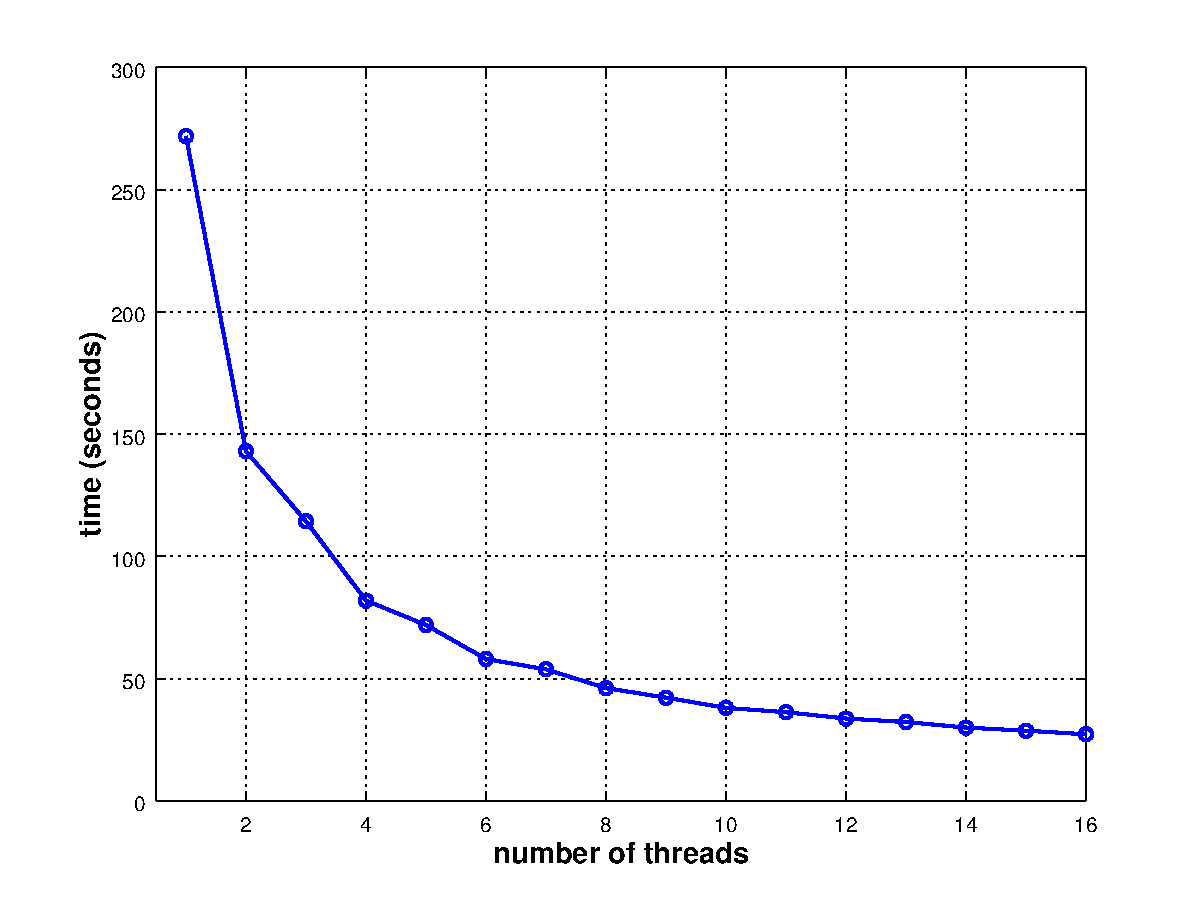
\includegraphics[width=1.1\textwidth]{plot1.pdf}\\
    {(a)}
  \end{minipage}%
  \begin{minipage}{0.5\textwidth}
    \centering
    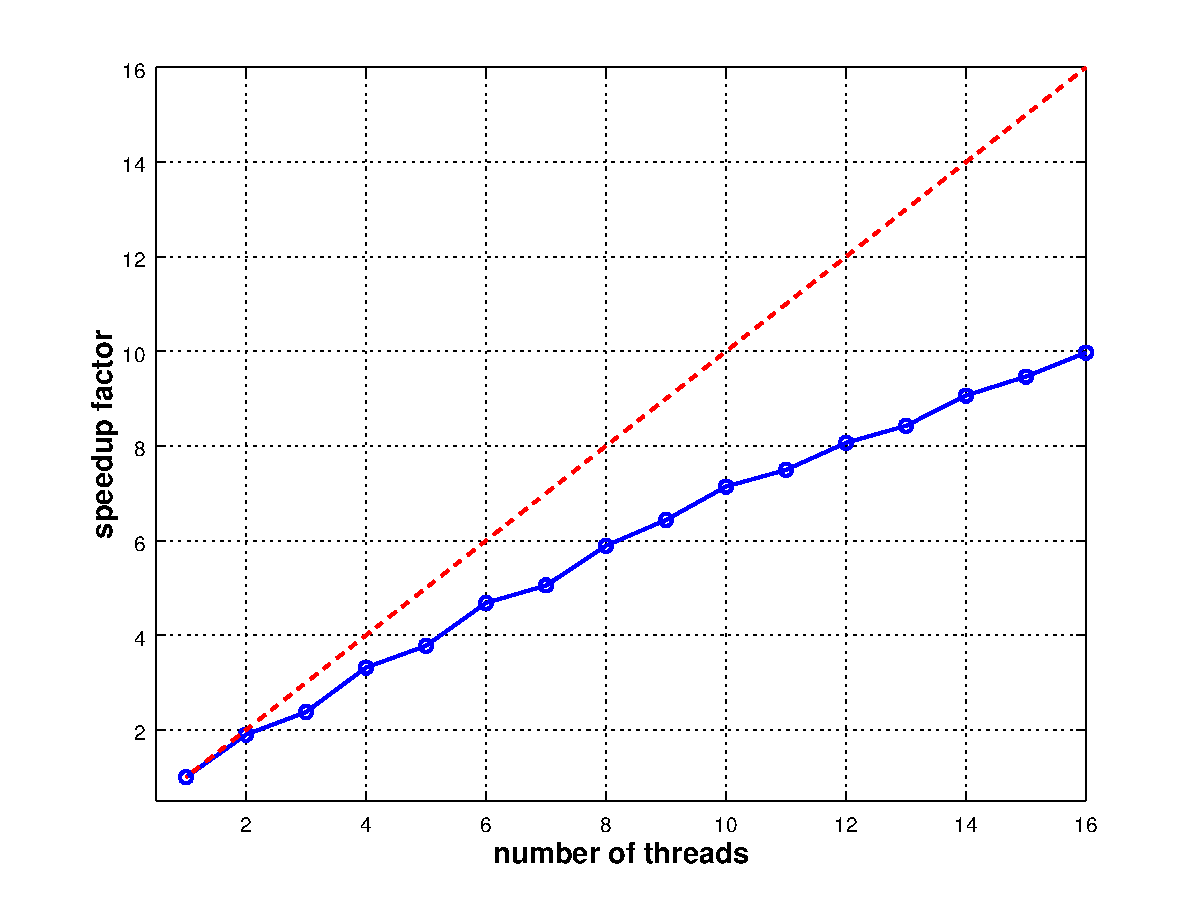
\includegraphics[width=1.1\textwidth]{plot2.pdf}\\
    {(b)}
  \end{minipage}
\end{minipage}
\caption
  {
  Execution characteristics for training a 100 component GMM
  to model a synthetic dataset comprising 1,000,000 samples with 100 dimensions,
  using 10 iterations of the {\it k}-means algorithm and 10 iterations of the EM algorithm:
  {\bf (a)}~total~time~taken depending on the number of threads;
  {\bf (b)}~corresponding speedup factor compared to using one thread (blue line), and idealised linear speedup under the assumption of no overheads and no memory access contention (red dotted line).
  The modelling was done on a machine with dual Intel Xeon E5-2620-v4 CPUs, providing 16 independent processing cores running at 2.1~GHz.
  Compilation was done with the GCC 5.4 C++ compiler using the following switches: \texttt{-O3 -march=native -fopenmp}.
  }
\label{fig:speedup}
\end{figure*}


\subsection{Comparison with Full-Covariance GMMs in MLPACK}

% I guess we should move the parallelism experiment here, if you go with this
% approach.

% This paragraph could be reworked---it doesn't really fit with the "flow" of
% the paper.  But I think it would be nice to show that using a diagonal GMM
% doesn't cost us too much---because that would be my primary concern as a
% reviewer (i.e. "this contribution doesn't matter because nobody uses diagonal
% GMMs").
In order to validate our intuition that a diagonal GMM is a good choice instead
of the significantly more complex problem of estimating GMMs with full covariance matrices,
we compare the {\it gmm\_diag} class (described in Section~\ref{sec:implementation})
against the full-covariance GMM implementation in the well-established MLPACK C++ machine learning library~\cite{Curtin_2013}.

We selected common datasets from the UCI machine learning dataset repository~\cite{Lichman_2013},
and trained both diagonal and full-covariance GMMs on these datasets.
The number of Gaussians was chosen according to the original source of each dataset;
where possible, 3 times the number of classes in the dataset was used.
In some cases, small amounts of Gaussian noise was added to the dataset to ensure
training stability of the full-covariance GMMs.
% It takes too long to do BIC on this, we don't have time.  We could handle it
% after reviews possibly?  Really the number of Gaussians does not matter
% anyway, we only care here about how long it takes.
Both implementations used 10 iterations of {\it k}-means for initialisation,
followed by running the EM algorithm until convergence or reaching a maximum of 250 iterations.
The entire fitting procedure was repeated 10 times, each time with a different random starting point.

The results are given in Table \ref{tab:results}, which shows the best log-likelihood of the 10 runs,
the average wall-clock runtime for the fitting,
as well as dataset information
(number of samples, dimensionality, and number of Gaussians used for modelling).
We can see that the diagonal GMM implementation in 
the {\it gmm\_diag} class provides speedups from one to two orders-of-magnitude
over the full-covariance implementation in \mbox{MLPACK}.
% The speedup is more pronounced the more dimensions there are in a dataset.
Furthermore, in most cases there is no significant loss in goodness-of-fit (as measured by log-likelihood).
% In one case ({\it ozone}) the goodness-of-fit is lower; we conjecture that using a larger $N_G$ for the {\it gmm\_diag} class will improve the accuracy of the model.
In several cases ({\it winequality}, {\it phy}, {\it covertype}, {\it pokerhand})
the log-likelihood is notably higher for the {\it gmm\_diag} class;
we conjecture that in these cases the diagonal covariance matrices are acting as a form of regularisation to reduce overfitting~\cite{Bishop_2006}.


\begin{table*}[!tb]
%\vspace{5ex}
\centering
\normalsize
\begin{tabular}{|l|c|c|c|c|c|c|c|c|}
\hline
\multirow{2}{*}{\bfseries dataset} & {\bfseries num.}    & {\bfseries num.} & {\bfseries num.}  & {\bfseries MLPACK}   & {\bfseries {gmm\_diag}} & $\sfrac{\mbox{\bfseries MLPACK}}{\mbox{\bfseries gmm\_diag}}$ & {\bfseries MLPACK}             & {\bfseries {gmm\_diag}}        \\
                                   & {\bfseries samples} & {\bfseries dims} & {\bfseries Gaus.} & {\bfseries fit time} & {\bfseries fit time}    & {\bfseries fit time ratio}                                    & {$\mathbf \log~p(X|\lambda) $} & {$\mathbf \log~p(X|\lambda) $} \\
\hline
  cloud       & {\tt ~~~~2,048} & {\tt 10} & {\tt ~5} & {\tt ~~~~1.50s} &  {\tt\bfseries ~0.14s} & {\tt ~10.7} & {\tt-~59.98{\tiny$\times$}10$^{\mathtt 3}$} & {\tt-~64.12{\tiny$\times$}10$^{\mathtt 3}$} \\
  ozone       & {\tt ~~~~2,534} & {\tt 72} & {\tt ~6} & {\tt ~~~~8.59s} &  {\tt\bfseries ~0.10s} & {\tt ~85.9} & {\tt-226.13{\tiny$\times$}10$^{\mathtt 3}$} & {\tt-307.95{\tiny$\times$}10$^{\mathtt 3}$} \\
  winequality & {\tt ~~~~6,497} & {\tt 11} & {\tt 30} & {\tt ~~~16.10s} &  {\tt\bfseries ~0.68s} & {\tt ~23.7} & {\tt-~47.12{\tiny$\times$}10$^{\mathtt 3}$} & {\tt-~15.85{\tiny$\times$}10$^{\mathtt 3}$} \\
  corel       & {\tt ~~~37,749} & {\tt 32} & {\tt 50} & {\tt ~~544.62s} &  {\tt\bfseries ~4.55s} & {\tt 119.7} & {\tt+~~4.52{\tiny$\times$}10$^{\mathtt 6}$} & {\tt+~~4.44{\tiny$\times$}10$^{\mathtt 6}$} \\
  birch3      & {\tt ~~100,000} & {\tt ~2} & {\tt ~6} & {\tt ~~~18.13s} &  {\tt\bfseries ~2.39s} & {\tt ~~7.6} & {\tt-~~2.70{\tiny$\times$}10$^{\mathtt 6}$} & {\tt-~~2.71{\tiny$\times$}10$^{\mathtt 6}$} \\
  phy         & {\tt ~~150,000} & {\tt 78} & {\tt 30} & {\tt ~3867.12s} &  {\tt\bfseries 29.25s} & {\tt 132.2} & {\tt-~~2.10{\tiny$\times$}10$^{\mathtt 7}$} & {\tt-~~1.88{\tiny$\times$}10$^{\mathtt 7}$} \\
  covertype   & {\tt ~~581,012} & {\tt 55} & {\tt 21} & {\tt 10360.53s} &  {\tt\bfseries 64.83s} & {\tt 159.8} & {\tt-~~9.46{\tiny$\times$}10$^{\mathtt 7}$} & {\tt-~~6.90{\tiny$\times$}10$^{\mathtt 7}$} \\
  pokerhand   & {\tt 1,000,000} & {\tt 10} & {\tt 25} & {\tt ~3653.94s} &  {\tt\bfseries 55.85s} & {\tt ~65.4} & {\tt-~~1.90{\tiny$\times$}10$^{\mathtt 7}$} & {\tt-~~1.68{\tiny$\times$}10$^{\mathtt 7}$} \\
\hline
\end{tabular}
\vspace{1ex}
\caption
  {
  Comparison of fitting time (seconds) and goodness-of-fit (as measured by log-likelihood) using full covariance GMMs from the MLPACK library~\cite{Curtin_2013}
  against diagonal GMMs in the {\it gmm\_diag} class,
  on common datasets from the UCI machine learning dataset repository~\cite{Lichman_2013}.
  The lower the fitting time, the better.
  The higher the $\log p(X|\lambda)$, the better.
  }
\label{tab:results}
\end{table*}


%% CS: I thought about the data you sent by email (matched results) and a good way to explain the story,
%% CS: but so far I haven'tt come up with something that was easy to grasp and didn't raise more questions.
%% CS: I think the way forward would be to choose a result from Table I (comparison against full cov GMM)
%% CS: where gmm_diag is getting a notably worse log-likelihood for the same N_G as the full cov GMM,
%% CS: and then see if the log-likelihood can be improved by increasing N_G.
%% CS: At that point we can compare the amout of time taken by full cov GMM and gmm_diag with higher N_G.

% Additionally, we perform a more detailed investigation of the behavior of each
% implementation on the {\tt corel} dataset.  In order to verify the results of
% Reynolds~\cite{Reynolds_2000}, we train diagonal and full-covariance GMMs on a
% variety of choices of $N_g$, collecting the log-likelihood of the trained model
% at each EM iteration.  This shows us how quickly each model is able to fit to
% the data.  Figure~\ref{fig:lc} shows the resulting learning curve, demonstrating
% that the diagonal GMM implementation is able to converge to a better
% log-likelihood in less time than the full-covariance implementation.
% 
% \begin{figure*}
% \begin{center}
% % This figure is horrible.  I have not thought of a better way to plot this
% % here.  But maybe it is a start.  Like for real this is the ugliest graph I
% % have ever produced in my life.
% % \includegraphics[width=\textwidth]{data/garbage_fire.png}
% \end{center}
% \caption{GMM training time vs. log-likelihood of model for diagonal GMMs (blue)
% and non-diagonal GMMs (red).  The simulation is performed for many values of
% $N_g$, showing that for the {\tt corel} dataset, we can get a faster and better
% fit with our implementation of diagonal GMMs than with a full-covariance GMM,
% even when the diagonal GMM must have a greater $N_g$ to achieve a better fit.}
% \label{fig:lc}
% \end{figure*}

% done with N_G = 30
% 
% birch     full        -2.5941e6       82.4212s
% birch     gmm_diag    -2.62008e6      8.1022s
% 
% phy       full        -2.36e7         5102.751s
% phy       gmm_diag    -7.94981e6      78.44s
% 
% covertype full        -1.09351e8      13221.844s
% covertype gmm_diag    -5.190e7        344.413s



% \begin{table*}[!tb]
% \vspace{5ex}
% \centering
% \small
% \begin{tabular}{|l|c|c|c|c|c|c|c|}
% \hline
% {\bf Dataset} & {\bf $N_v$} & {\bf dims} & {\bf $N_g$} & {\bf MLPACK fit time} & {\bfseries {\it\bfseries gmm\_diag} fit time} & {\bf MLPACK $\log(p(X|\lambda))$} & {\bf {\it\bfseries gmm\_diag} $\log(p(X|\lambda))$} \\
% \hline
%   cloud       & ~~2,048 & 10 &  5 & ~~~~~1.375s & ~~~{\bf 0.164s} & $-59.9  \times 10^{3}$ & $-63.0  \times 10^{3}$ \\
%   ozone       & ~~2,534 & 72 &  6 & ~~~~~1.982s & ~~~{\bf 0.202s} & $-230   \times 10^{3}$ & $-399   \times 10^{3}$ \\
%   winequality & ~~6,497 & 11 & 30 & ~~~~18.201s & ~~~{\bf 1.257s} & $-47.5  \times 10^{3}$ & $-15.6  \times 10^{3}$ \\
%   corel       & ~37,749 & 32 & 50 & ~~~501.601s &  ~{\bf 22.016s} & $~~2.99 \times 10^{6}$ & $~~2.89 \times 10^{6}$ \\
%   cup98b      & ~95,413 & 56 & 30 &  ~1207.860s &  ~{\bf 48.425s} & $-11.9  \times 10^{6}$ & $-6.62  \times 10^{6}$ \\
% % birch3      & 100,000 & 2  &  6 & \\
%   birch3      & 100,000 & ~2 & 30 & ~~~~82.421s &  ~~{\bf 8.102s} & $-2.59  \times 10^{6}$ & $-2.62  \times 10^{6}$ \\
%   phy         & 150,000 & 78 & 30 &  ~5102.751s &  ~{\bf 78.440s} & $-2.36  \times 10^{7}$ & $-7.94  \times 10^{6}$ \\
% % covertype   & 581,012 & 55 & 21 & \\
%   covertype   & 581,012 & 55 & 30 &  13221.844s &  {\bf 344.413s} & $-1.09  \times 10^{8}$ & $-5.19  \times 10^{7}$ \\
% % pokerhand   & 1000000 & 10 & 25 & 30 & \\
% \hline
% \end{tabular}
% \caption
%   {
%   Comparison of fitting time (seconds) and goodness-of-fit (as measured by log-likelihood) using full covariance GMMs from the MLPACK library~\cite{Curtin_2013}
%   against diagonal GMMs in the {\it gmm\_diag} class,
%   on common datasets from the UCI machine learning dataset repository~\cite{Lichman_2013}.
%   $N_v$ indicates the number of samples, {\it dims} indicates dimensionality, and $N_G$ the number of Gaussians.
%   }
% \label{tab:results}
% \end{table*}

% \begin{table*}
% \begin{center}
% \begin{tabular}{|l|c|c|c|c|c|c|c|}
% \hline
% {\bf dataset} & {\bf $N_v$} & {\bf dims} & {\bf $N_g$} & {\bf full-covariance fit time} & {\bf Armadillo fit time} & {\bf full-diagonal $\log(p(X|\lambda))$} & {\bf Armadillo $\log(p(X|\lambda))$} \\
% \hline
% cloud & 2048 & 10 & 5 & 1.375s & {\bf 0.164s} & -59.9k & -63.0k \\
% ozone & 2534 & 72 & 6 & 1.982s & {\bf 0.202s} & -230k & -399k \\
% winequality & 6497 & 11 & 30 & 18.201s & {\bf 1.257s} & -47.5k & -15.6k
% \\
% corel & 37749 & 32 & 50 & 501.601s & {\bf 22.016s} & 2.99M & 2.89M \\
% cup98b & 95413 & 56 & 30 & 1207.86s & {\bf 48.425s} & -11.9M & -6.62M \\
% birch3 & 100000 & 2 & 6 & \\
% phy & 150000 & 78 & 30 & & {\bf 78.44s} & & -7.94M \\
% covertype & 581012 & 55 & 21 & \\
% pokerhand & 1000000 & 10 & 25 & 30 & \\
% \hline
% \end{tabular}
% \end{center}
% \caption{Datasets used for comparisons with full-covariance GMM estimation.}
% \label{tab:results}
% \end{table*}

% \begin{table*}
% \begin{center}
% \begin{tabular}{|l|c|c|c|c|c|c|c|}
% \hline
% {\bf dataset} & {\bf $N_v$} & {\bf dims} & {\bf $N_g$} & {\bf
% full-covariance fit time} & {\bf Armadillo fit time} & {\bf full-diagonal
% $\log(p(X|\lambda))$} & {\bf Armadillo $\log(p(X|\lambda))$} \\
% \hline
% cloud & 2048 & 10 & 5 & 1.375s & {\bf 0.164s} & -59.9k & -63.0k \\
% ozone & 2534 & 72 & 6 & 1.982s & {\bf 0.202s} & -230k & -399k \\
% winequality & 6497 & 11 & 30 & 18.201s & {\bf 1.257s} & -47.5k & -15.6k \\
% corel & 37749 & 32 & 50 & 501.601s & {\bf 22.016s} & 2.99M & 2.89M \\
% cup98b & 95413 & 56 & 30 & & {\bf 48.425s} &  & -6.62M \\
% birch3 & 100000 & 2 & 6 & \\
% phy & 150000 & 78 & 30 & \\
% covertype & 581012 & 55 & 21 & \\
% pokerhand & 1000000 & 10 & 25 & 30 & \\
% \hline
% \end{tabular}
% \end{center}
% \caption{Datasets used for comparisons with full-covariance GMM estimation.}
% \label{tab:results}
% \end{table*}

